

\documentclass[8pt]{article}

\usepackage[utf8]{inputenc}

\usepackage{amsmath}
\usepackage{graphicx}
\usepackage{amssymb}
\usepackage{float}
% set font size to 11pt


\setlength{\parskip}{\baselineskip}%
\setlength{\parindent}{0pt}%

\begin{document}

\begin{figure}[h]
    \centering
    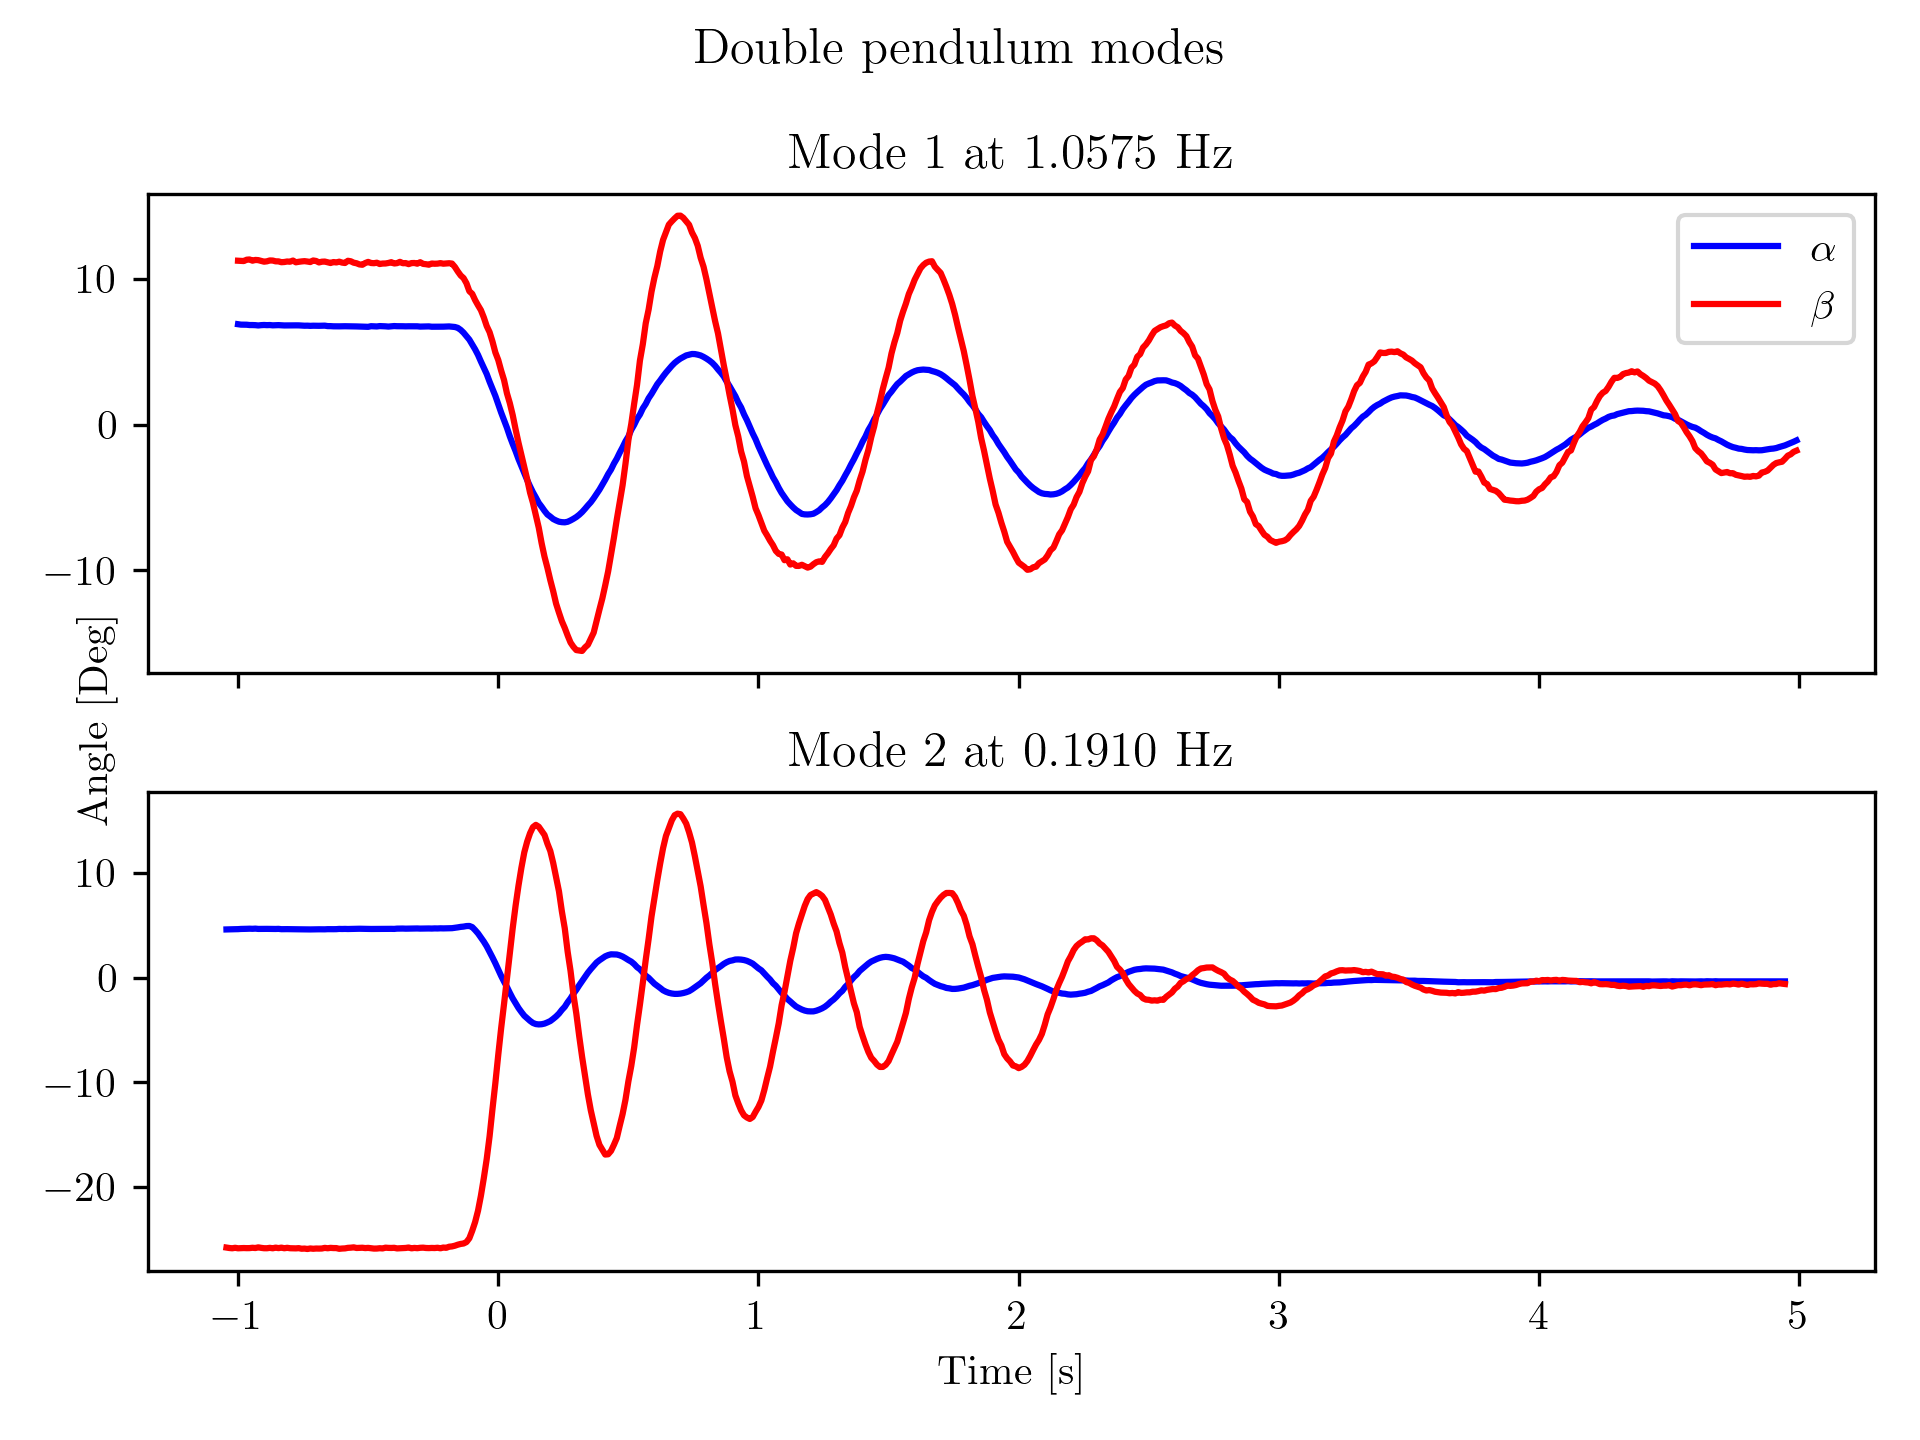
\includegraphics[width=1\textwidth]{modes.png}
    \caption{Mode shapes of the double pendulum}
    \vspace{-1pt}
    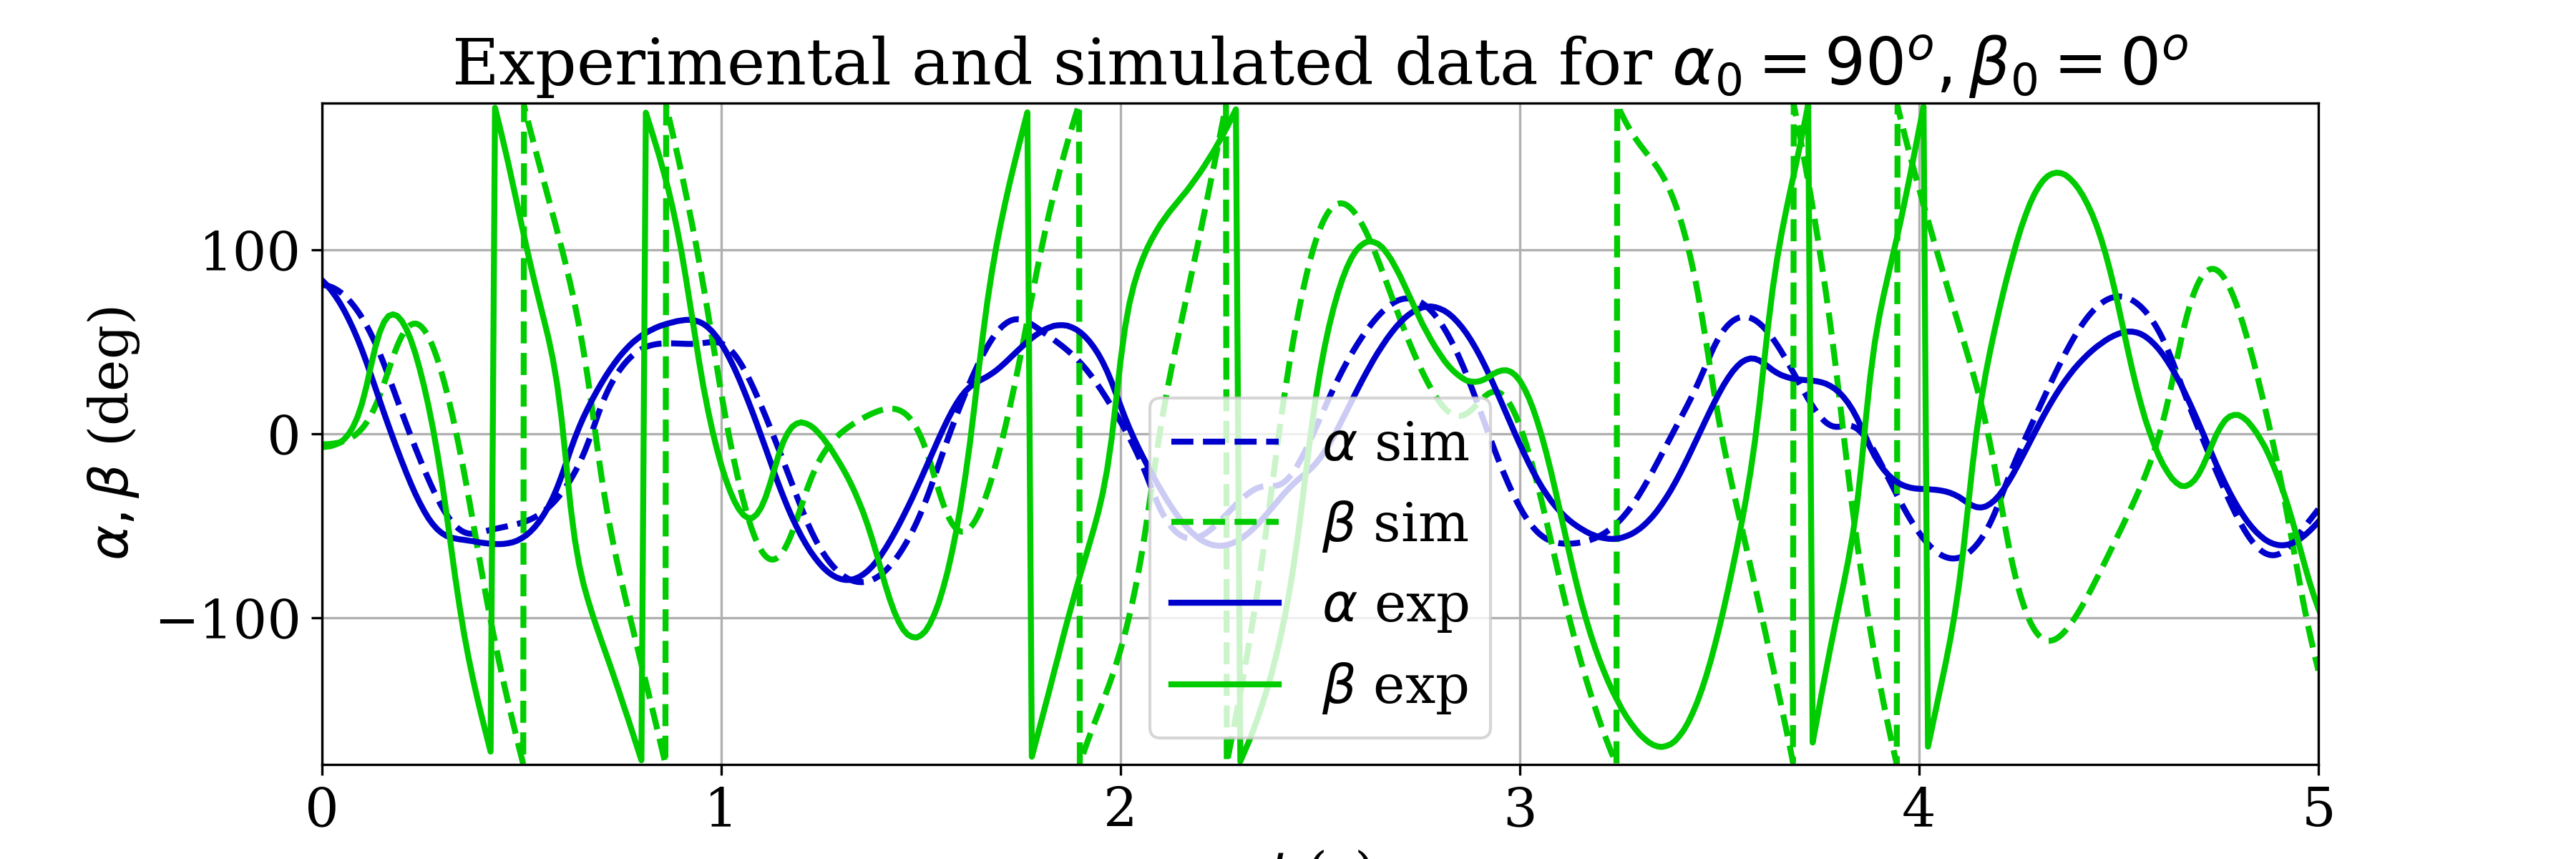
\includegraphics[width=1\textwidth]{EP_4_exp_sim.png}
    \caption{Plot of Experimental and simulated values for $\alpha$ and $\beta$ against time for $\alpha_0 = 90^{\circ}$, $\beta_0 = 0^{\circ}$}
\end{figure}

\begin{figure}[h]
    \centering
    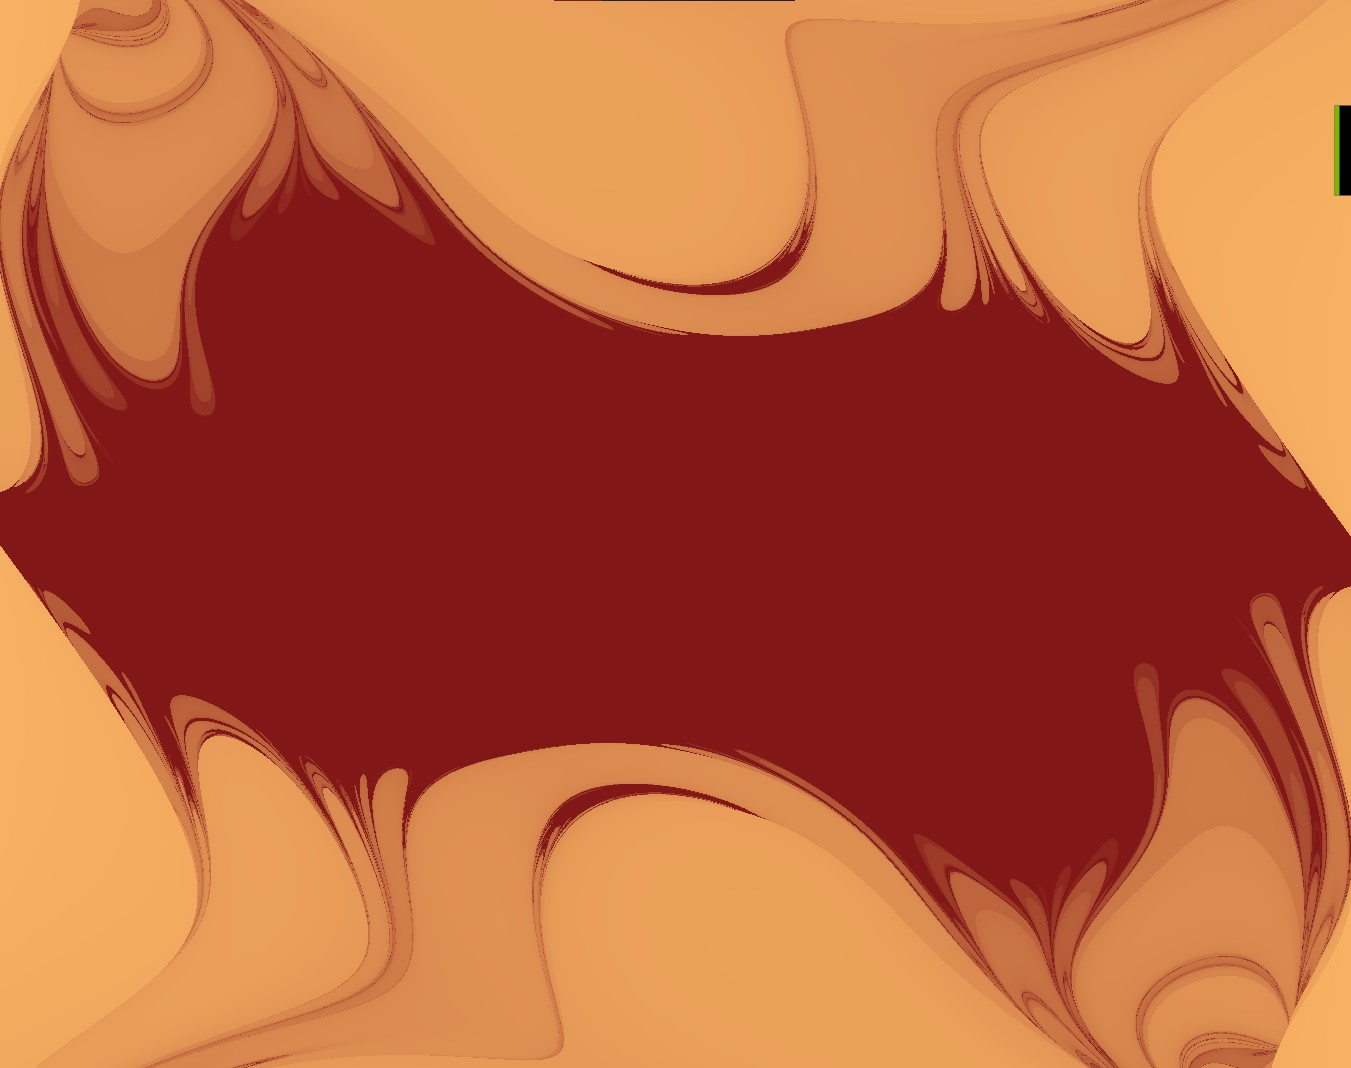
\includegraphics[width=1\textwidth]{time_of_flip_render.jpg}
    \caption{Fractal of the time of flip produced by a modified Julia rendering algorithm using SFML}
\end{figure}


\vspace{-2cm}

\end{document}